\section{Project Development}

This section details the development of Pookie, an AI-driven robot designed to promote mental wellbeing, developed under design supervision from Chula Student Wellness, a platform for free psychological counseling for Chula students. Pookie aims to act as a companion to help alleviate feelings of stress and anxiety, especially in response to future societal concerns like ”Terror Outbursts,” an anxiety-driven phenomenon anticipated to affect Thailand. The project focuses on enhancing positivity and emotional attachment by creating a robot that interacts with users in an empathetic and calming manner.

\subsection{Overview}
\begin{figure}[!htb]
    \centering
    \captionsetup{justification=centering}
    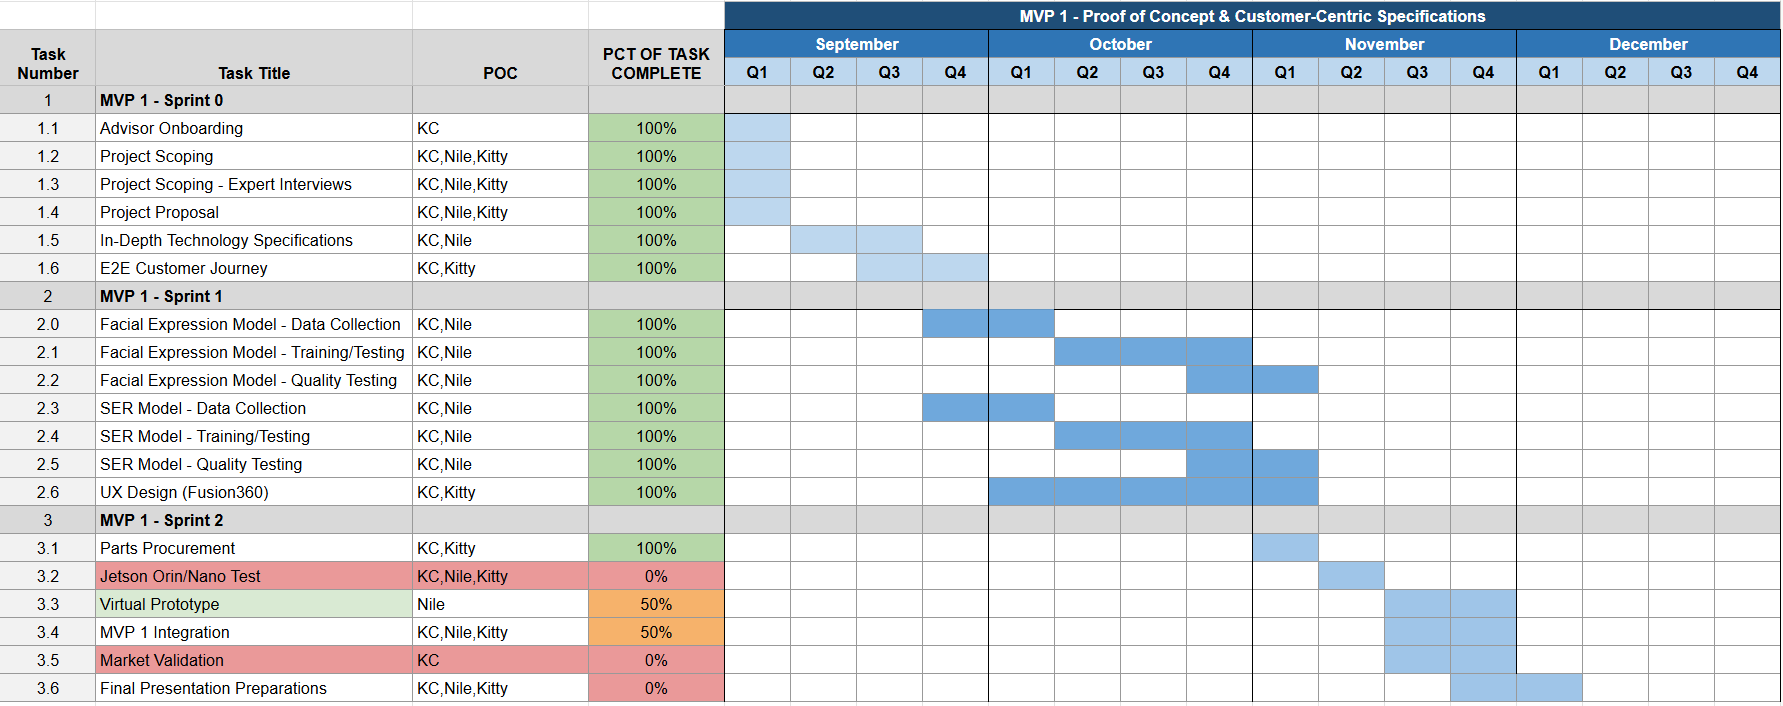
\includegraphics[width=\textwidth]{gantt.png}
    \caption{Project GANTT Chart}
    \label{fig:gantt}
\end{figure}

The project comprises a total of two scopes, one for each semester, where each scope will have its respective expectations. The two scopes are MVP 1 (Proof of Concept) and MVP 2 (Market Prototype). In general, MVP 1 aims to initially collect specifications and design inspiration through primary (expert interviews) and secondary research. Next, a minimum viable product including a working set of AI algorithms, software integration, and CAD mockup was created. On the other hand, MVP 2 aims to elevate the proof of concept to a market prototype, where the software aspects such as AI and integration would be quality tested and dynamic, and the hardware would be readily available for testing.

This report details the implementation of Pookie MVP 1 (Proof of Concept) over the span of four months in semester one. Overall, the project has taken the correct trajectory since conceptualization. As shown in Figure 3, MVP 1 comprises three sprints (Sprint 0, Sprint 1, Sprint 2). In Sprint 0, the team focused on overall product design, reaching out to Dr. Kunparinya Siripanit from Chula Student Wellness for top-down design specifications to accommodate users of general anxiety. Additionally, the team spent time addressing feasibility aspects of the project and literature review, which was discussed in the project proposal. Next, in Sprint 1, the team split into working on their respective tasks, where the software engineering members researched and trained AI models on emotion recognition, including speech emotion recognition and facial emotion recognition, whereas the hardware engineering team focused on developing a mockup of the robot’s physical appearance and acquiring necessary pieces of equipment. Finally, in Sprint 2, the team attempted to integrate all fundamental pieces of software and hardware together. While the project expected integration of software with the Jetson Orin microcomputer, it was recommended by Dr.Paulo instead to focus on developing a virtual prototype, to which a Fusion360 render of the robot’s basic interactions and movements were created. Additionally, the task of \textit{market validation} was also canceled, where initially it was planned that a customer survey and customer interview would be collected to obtain further feedback and refine Pookie’s concept.

\newpage
\subsection{Design Concept}

\subsubsection{Design Reference}

This section illustrates the overall design concept and references for Pookie. Pookie, the emotional wellbeing robot, is conceptualized as a responsive, AI-driven companion designed
to improve mental well-being, specifically catered to customers under the influence of stress and anxiety. To be specific, anxiety in this project is indicated by signs of stress or worry, and the definition of \textit{emotional wellbeing} is \textit{positivity promotion}. It is important to note that the scope of the project, in terms of emotional support, is identified as \textit{promotion}, meaning promotion of positive wellbeing through the use of robotics, rather than \textit{prevention}, which refers to a specific goal of preventing long term issues such as depression or suicide.

With Pookie, it was advised by Dr. Fah Kunpariya (Counseling Psychologist from Chula Student Wellness) to implement an animal-like design with anthropomorphic features. The reason is to reference designs that stimulate a sense of calmness, such as a pet-like design. As such, Pookie resembles a teddy bear, which hopes to stimulate the user with a sense of calmness and childhood nostalgia. After brainstorming and conceptualization, a Fusion360 CAD mockup for Pookie was created. Pookie’s outer shell was 3D printed to hide and house a series of motors, microcontrollers and other necessary electronic components as illustrated in Figure N. Within the scope of this semester, the hardware aspects only comprised a Fusion360 CAD Mockup and virtual prototype. Physical hardware assembly and complete integration was expected to be out of scope, and will begin early next semester in MVP2.

\begin{figure}[!htb]
    \centering
    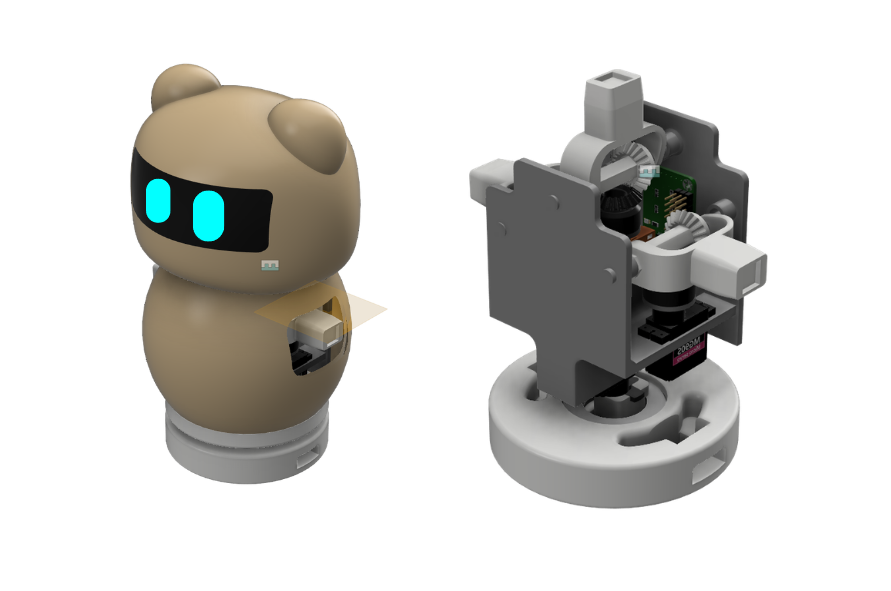
\includegraphics[width=0.7\textwidth]{compare.png}
    \caption{Pookie CAD Mockup. \textit{Left:} Physical Appearance Design, \textit{Right:} Internal Hardware Design.}
    \label{fig:comparison}
\end{figure}

\subsection{Limitations and Scope}

This project aims to develop a proof of concept for an emotional well-being robot, drawing inspiration from existing models such as Kiki. However, there are several limitations and scope considerations for this project:

\begin{itemize}
    \item \textbf{Security:} The primary focus of this project is to create a prototype that demonstrates the feasibility of an emotional well-being robot. As such, the security measures implemented will be at a basic level. Comprehensive security features, including data encryption and advanced user authentication, are beyond the scope of this project.
    \item \textbf{Safety:} While the robot will undergo rigorous testing to ensure fundamental safety in terms of electronics, heat output, and physical design, the scope of safety considerations will be limited to these basic aspects. Detailed safety protocols, including long-term durability and fail-safes for unforeseen hazards, will not be extensively addressed in this prototype phase.
    \item \textbf{Functionality:} The robot will focus on core emotional well-being functionalities, such as basic interaction and mood assessment. Advanced features, such as personalizing therapeutic interventions or integration with external health systems, will not be included in this prototype.
    \item \textbf{User Experience:} The prototype will provide a foundational user experience but may lack the polish and customization of fully developed models. User interface and experience enhancements will be considered in future, scaled development phases.
    \item \textbf{Scalability:} The project will not address scalability concerns for mass production or widespread deployment. The prototype is intended to demonstrate initial concepts and feasibility rather than full scale implementation.
    Integration: This project will not explore extensive integration with other technologies or platforms. The focus will remain on the standalone capabilities of the robot, with minimal emphasis on interoperability with existing systems.
    
\end{itemize}

By acknowledging these limitations and scope considerations, this project sets clear expectations and defines the boundaries of its initial development phase. Future iterations may address these areas in greater detail based on feedback and further research.

\subsection{Software Implementation}
Software implementation for Pookie comprises two key pillars: emotion detection and interaction. Emotion detection is an initiative to incorporate empathy for the customer experience with the robot, using computer vision to analyze facial expressions, as well as speech emotion recognition to analyze tone and pitch. For each AI model, the robot utilizes feature labels of the seven universal emotions (happiness, neutral, sadness, fear, anger, disgust, surprise), which are used as a baseline for many emotion classification tasks, including stress and anxiety detection. In particular, stress and anxiety symptoms are shown to be associated with negative emotions being fear, disgust, and anger, as discussed with Dr.Fah Kunpariya, our psychology advisor. Given predicted emotional status, the robot will be programmed to provide interaction in two forms: verbal and non-verbal. Verbal interactions consist of noises made by the robot, whereas nonverbal interactions comprise physical actions from the robot such as arm movement changes in the LED display resembling its eyes. 
In terms of progress, the goal for semester one was a minimum viable software product, comprising two working AI models and an integration backend that combines the with physical actions and other processing. In terms of AI model implementation, the facial emotion recognition and speech emotion recognition models produced decent results, being more than 50\% accurate in all emotions’ classifications. The integration of these two models uses a server-client architecture to deliver physical interaction, which will be discussed in the software architecture section.

\subsubsection{Process Flowchart}
The process flowchart for Pookie MVP 1 is illustrated in Fig. \ref{fig:flowchart}. Overall, Pookie will detect the user’s face and voice and process the input to induce an action. Based on the emotions detected, such as happy, sad, or negative emotions (inferred as stress), then Pookie will carry out a set of physical actions, including sound, eyes, and actuator. 

\begin{figure}[ht]
    \centering
    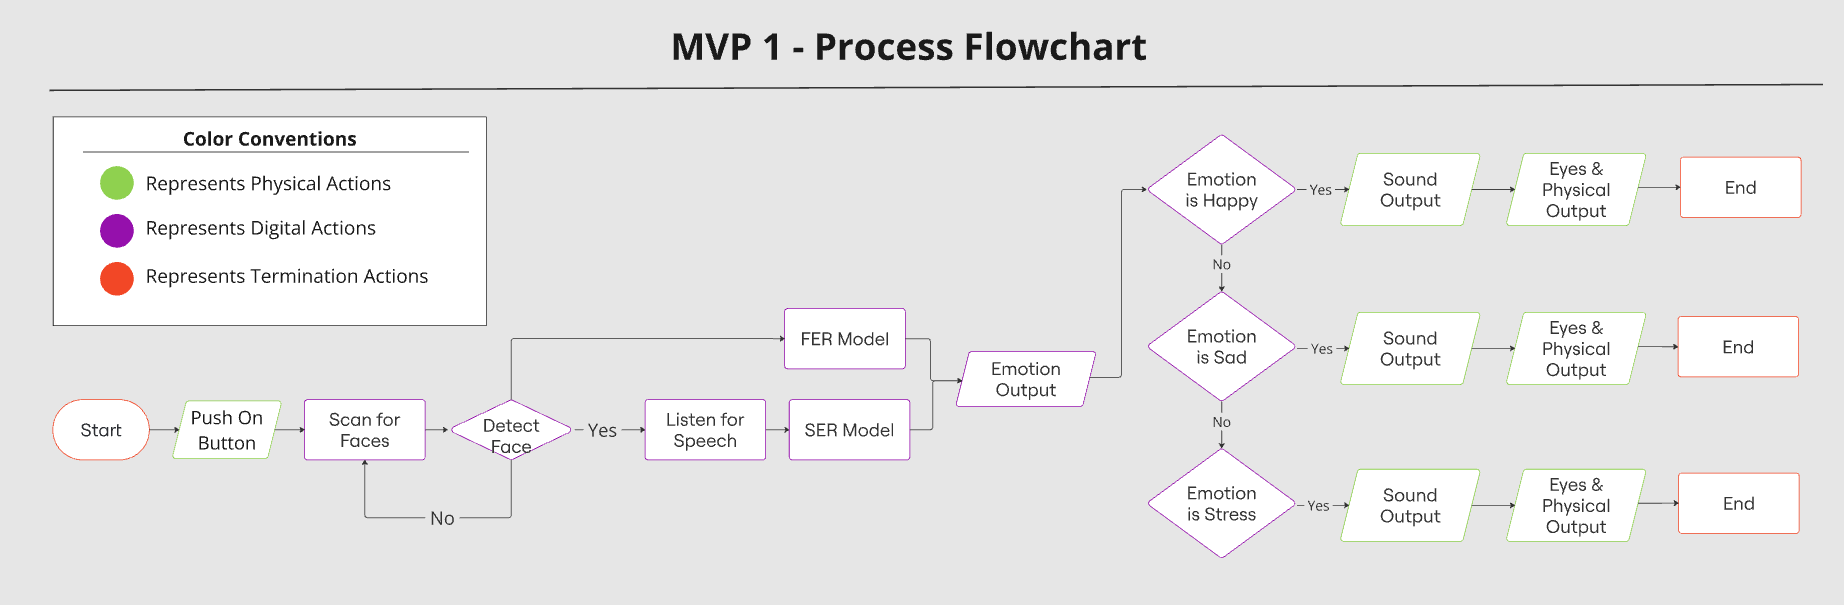
\includegraphics[width=\textwidth]{flowchart.png}
    \caption{MVP 1 Process Flowchart}
    \label{fig:flowchart}
\end{figure}

\subsubsection{Software Architecture and Integration}
To go into further detail on the process flowchart, this section illustrates the solution architecture, involving core technologies used, including servers, clients, libraries and so on.
\textbf{System Overview}

The architecture employs a three-tier structure consisting of:
\begin{itemize}
\item\textbf{Data Acquisition Layer:} Interfaces with sensors and hardware for input collection (e.g., facial images and voice).

\item\textbf{Processing Layer:} Handles emotion analysis using AI models and decision-making algorithms.

\item\textbf{Interaction Layer:} Manages the robot's responses, including audio, visual, and physical movements.
\end{itemize}

This layered design ensures that each module operates independently, facilitating parallel development and easier debugging.

\begin{figure}[ht]
    \centering
    \captionsetup{justification=centering}
    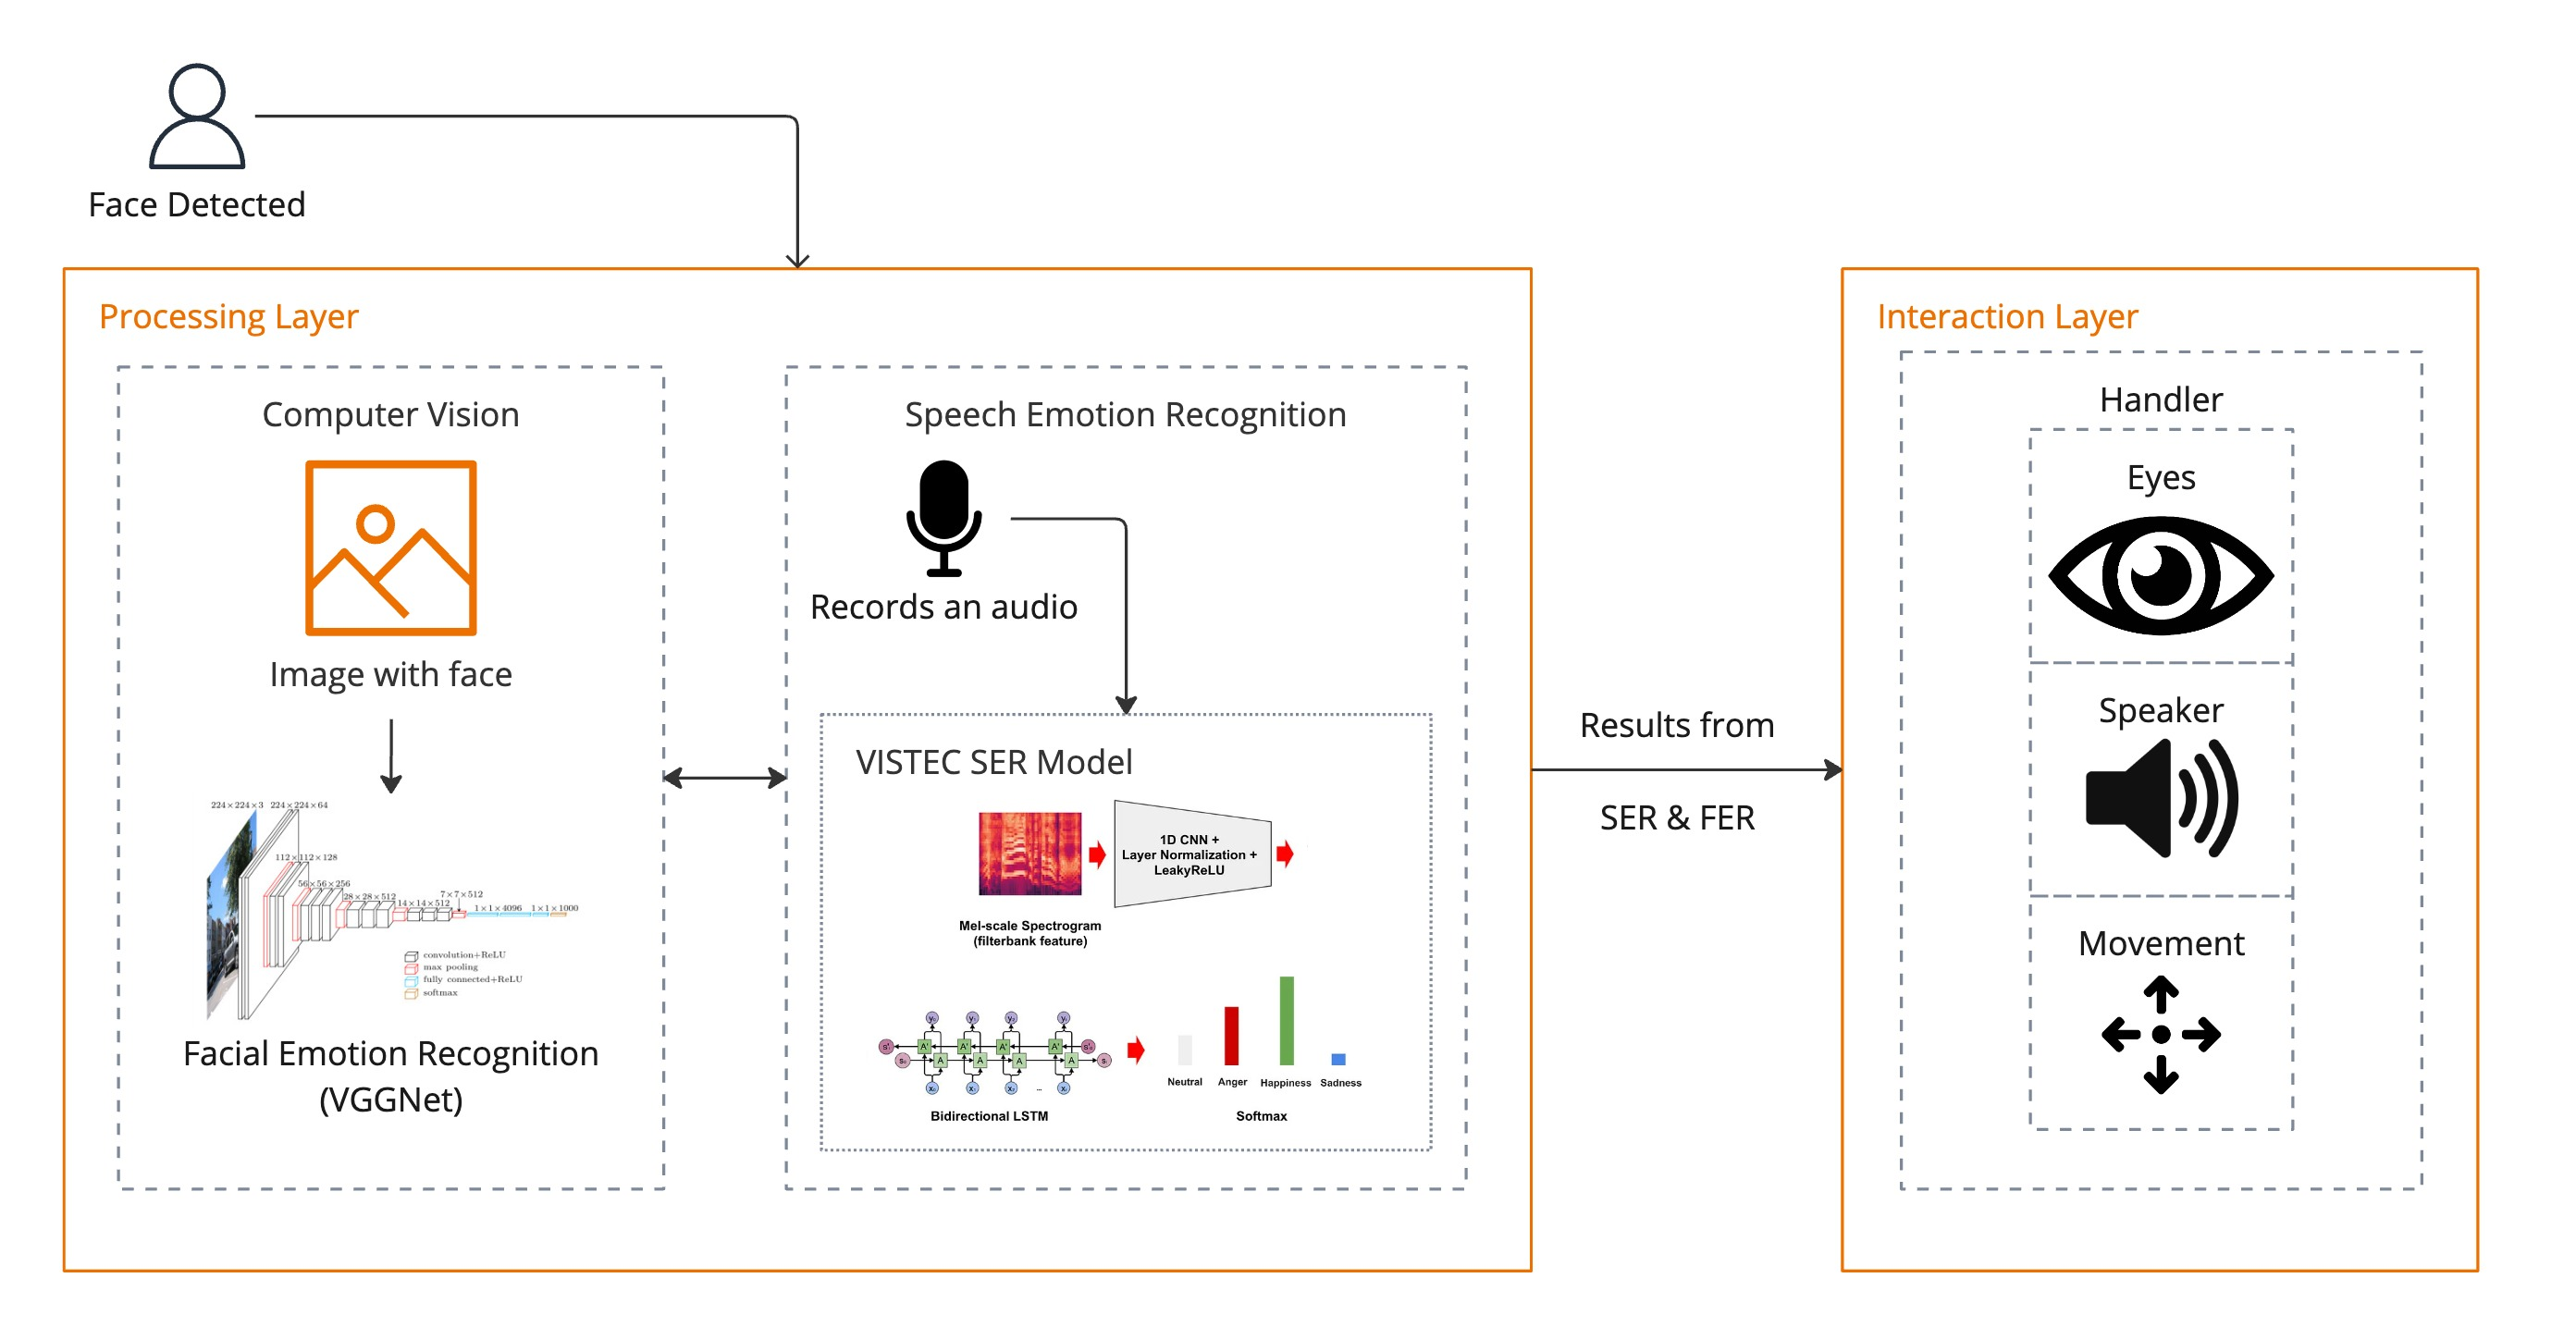
\includegraphics[width=\textwidth]{Flowchart.jpg}
    \caption{Pookie Software Architecture}
    \label{fig:architecture}
\end{figure}

\subsubsection{Key Components}
\begin{enumerate}
    \item\textbf{Emotion Detection Module}

    This module is responsible for identifying the user's emotional state based on facial expressions and speech patterns.
    \begin{itemize}
        \item\textbf{Facial Emotion Recognition (FER):} Utilizes a fine-tuned VGGNet model trained on the Chinese Faces Dataset. It processes real-time video feeds to classify emotions such as happiness, sadness, and stress.
        \item\textbf{Speech Emotion Recognition (SER):} Leverages a pre-trained model developed in collaboration with VISTEC, analyzing voice inputs for tonal features like pitch and intensity to detect emotions.
    \end{itemize}
    Both components output structured emotion data to the Core Integration Framework for further processing.
\item\textbf{Interaction Module}
    
    The Interaction Module generates empathetic responses based on detected emotions:
    \begin{itemize}
        \item\textbf{Verbal Interactions:} Uses pre-recorded audio and tone synthesis to produce comforting sounds or words.
        
        \item\textbf{Non-Verbal Interactions:} Controls physical actions such as arm movements, eye animations on the LED display, and body rotation using servo motors.
    \end{itemize}
\end{enumerate}
        

\subsubsection{Core Integration Framework}


This middleware orchestrates communication between the emotion detection and interaction modules. Key responsibilities include:
\begin{itemize}
    \item Synchronizing data streams from the FER and SER modules.
    \item Deciding responses using a rule-based system or decision tree logic.
    \item Triggering corresponding interaction commands.
\end{itemize}

\subsubsection{Component Interaction}

The interaction between components is depicted in the process flowchart. The steps include:
\begin{enumerate}
    \item\textbf{Data Acquisition:} Real-time inputs (video and audio) are captured using a USB camera and a lavalier microphone.
    \item\textbf{Emotion Detection:} Data is processed by FER and SER modules to output an emotional state.
    \item\textbf{Decision Making:} The Core Integration Framework maps the detected emotion to predefined response rules.
    \item\textbf{Response Execution:} Interaction Module activates verbal and non-verbal responses.
\end{enumerate}

\subsection{Facial Emotion Recognition}
The development of the AI-driven robot incorporates a crucial element: detecting and interpreting user emotions, particularly stress and anxiety, using Facial Emotion Recognition (FER). In particular, stress will be mapped to negative emotions: fear, anger, and disgust.

\subsubsection{Faces Dataset}
The facial expression recognition model was trained on a Chinese Faces Dataset , chosen for its similar characteristics to the hard-to-obtain Thai dataset. Utilizing an intuitive approach to synthetic data generation, the dataset was based on a  \textbf{Chinese Face Dataset with Dynamic Expressions and Diverse Ages Synthesized by Deep Learning} \cite{han-2023}, where a team of researchers created a facial expression image generation model for various Chinese faces belonging to different age groups, genders, and face structure, as shown in Figure \ref{fig:face}, labeled as “Ours”.

\begin{figure}[ht]
    \centering
    \captionsetup{justification=centering}
    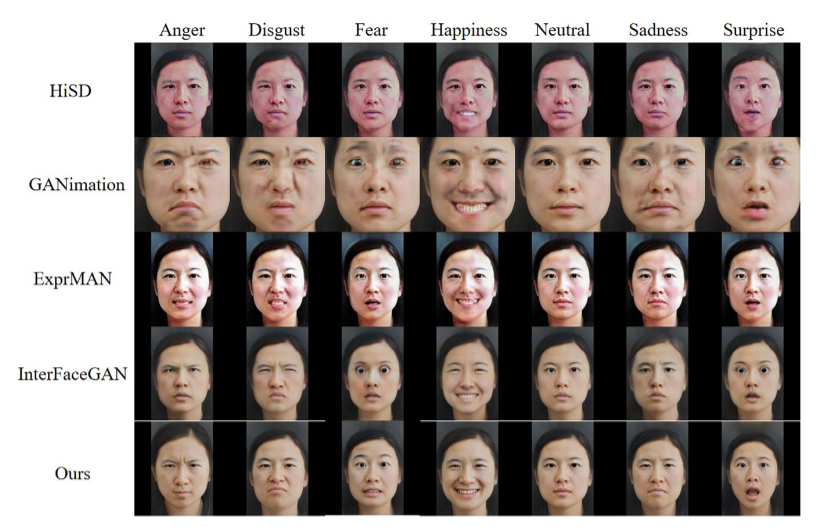
\includegraphics[width=\textwidth]{faces.png}
    \caption{ A Chinese Face Dataset with Dynamic Expressions and Diverse Ages Synthesized. Source: Adapted from \cite{han-2023}}
    \label{fig:face}
\end{figure}


\newpage
\subsubsection{Facial Emotion Recognition Model Development}
Initially, the facial expression recognition model for this project was expected to use a model fine tuning approach over a Chinese Faces Dataset, as it provides the most symmetric resemblance to a Thai dataset, which is difficult to obtain. For our approach, we took a pre-trained model for emotion recognition using VGGNet architecture, then fine tuned the inference layers on a Chinese dataset in order to get more accurate representation for Thai faces. The other layers were frozen, and served as foundation parameters for transfer learning. After multiple versions of the model, however, it could be seen that this approach did not yield great results. As shown in Figure \ref{fig:fer-dev}, the model yielded results far worse than simple guessing, most likely due to inappropriate usage of transfer learning on an already imperfect model.

\begin{figure} [!htb]
    \centering
    \captionsetup{justification=centering}
    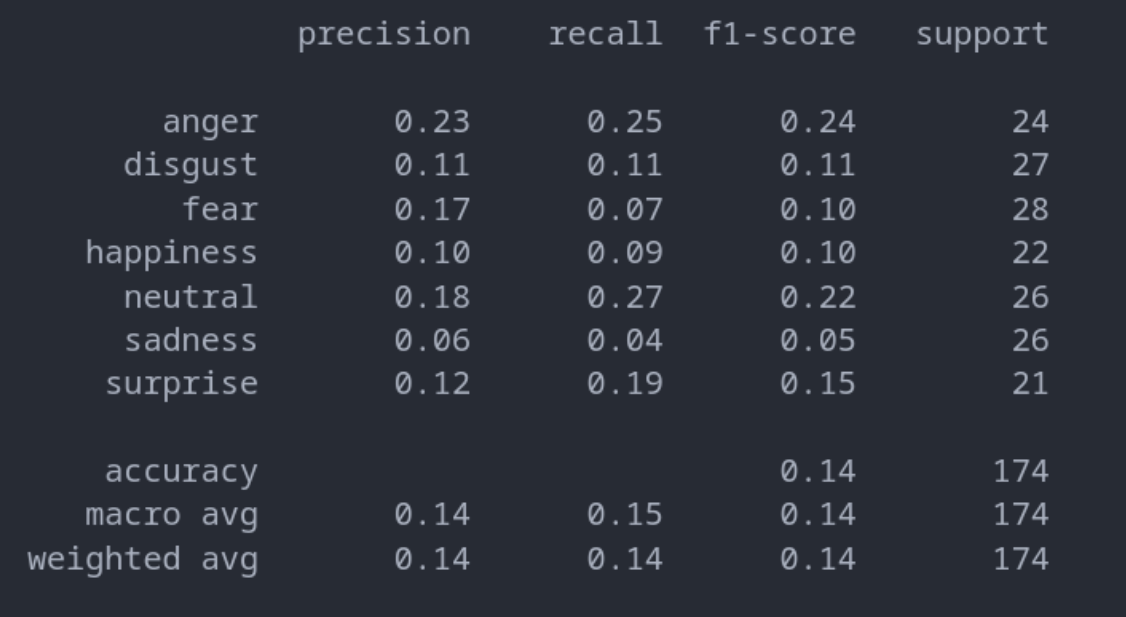
\includegraphics[width=\textwidth]{fer-dev.png}
    \caption{Initial Model Training Results}
    \label{fig:fer-dev}
\end{figure}

\subsubsection{Facial Emotion Recognition Model}
Utilizing a VGGNet \cite{simonyan2015deepconvolutionalnetworkslargescale} architecture (Figure \ref{fig:vgg}) —a multi-layer convolutional neural network renowned for feature extraction and classification, particularly in emotion detection models—the research aimed to develop an accurate facial recognition approach. The Chinese faces dataset was trained over the VGGNet architecture with little hyperparameter tuning.

As seen in the results, the model is great at distinguishing between positive emotions such as happiness or surprise, but it is quite lacking in negative emotions. However, given the scope of the project, where positive and neutral are associated with specific outputs, and negative emotions are all classified as stress, then the model is generally enough to use as a minimum viable product for the rest of the semester.

\begin{figure}
    \centering
    \captionsetup{justification=centering}
    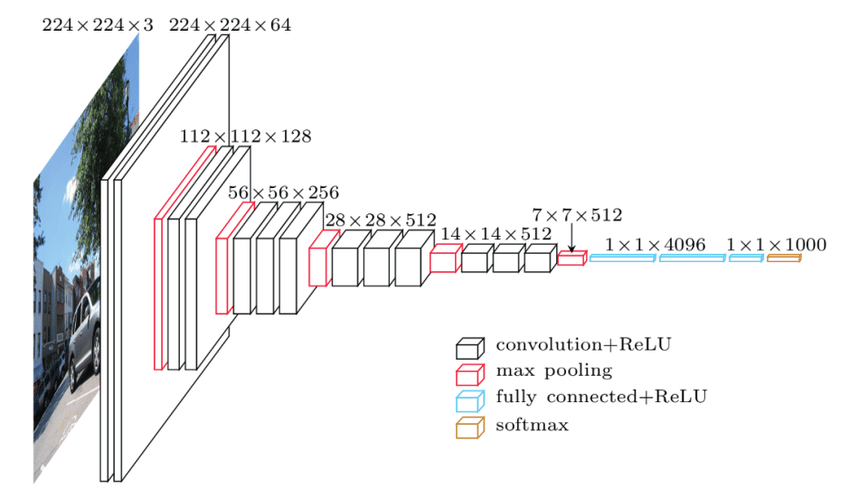
\includegraphics[width=0.8\textwidth]{vgg.png}
    \caption{VGGNet Architecture}
    \label{fig:vgg}
\end{figure}

\begin{figure}
    \centering
    \captionsetup{justification=centering}
    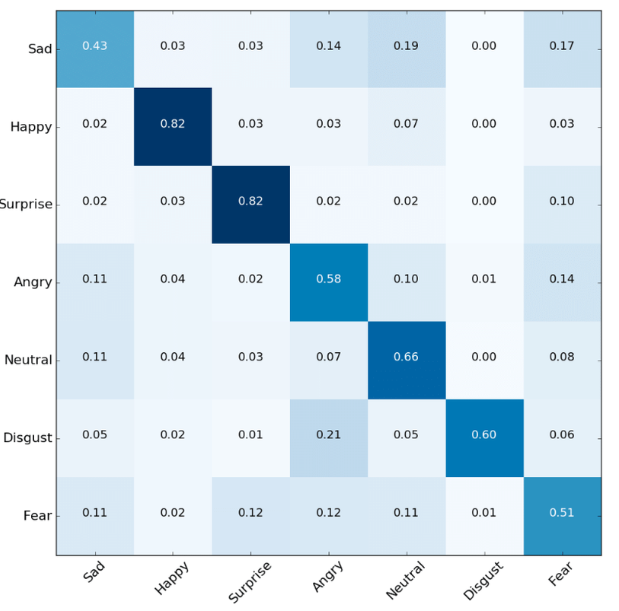
\includegraphics[width=0.8\textwidth]{fer_confusion.png}
    \caption{Validation Set Confusion Matrix}
    \label{fig:fer-con}
\end{figure}

\newpage
\subsection{Speech Emotion Recognition}
A key element of Pookie’s AI is the Speech Emotion Recognition (SER) system, which is used for recognizing the user’s emotions based on vocal patterns. By analyzing factors such as pitch, tone, and intensity, the system detects emotions: neutral, anger, happiness, sadness, and frustration. This section outlines the results and challenges faced during the implementation of the  speech emotion recognition model, starting with relevant datasets and methodologies.

\subsubsection{Speech Emotion Recognition Dataset and Model}
We are utilizing a dataset created by Chulalongkorn University in collaboration with VISTEC, DEPA, and AIS, containing 41 hours and 36 minutes of audio recordings labeled with five emotions: neutral, anger, happiness, sadness, and frustration.
The SER model used within Pookie is also developed by VISTEC which is a speech emotion recognition model based on the aforementioned dataset. 

The confusion matrix visualizes the performance of an emotion recognition model across five classes: neutral, anger, happiness, sadness, and frustration. The diagonal elements indicate correct predictions, with the highest accuracies being for neutral (0.72), anger (0.73), and frustration (0.61). Sadness and happiness show slightly lower accuracies at 0.6 and 0.62, respectively. However, some significant misclassifications occur, such as frustration being confused with sadness (0.31) and happiness being confused with frustration (0.17). The model's weighted accuracy is 66.12\%, while its unweighted accuracy is 65.67\%, reflecting a modest overall performance with some variability in recognizing different emotions accurately.

\begin{figure} [!htb]
    \centering
    \captionsetup{justification=centering}
    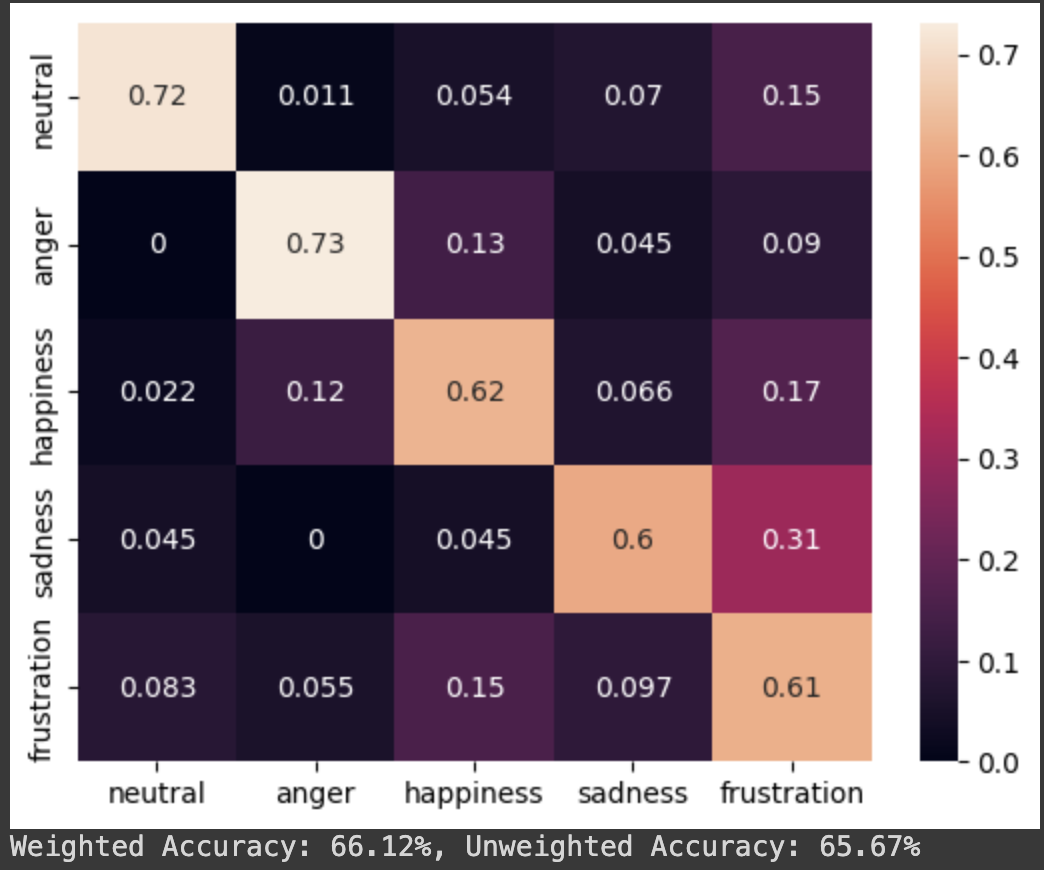
\includegraphics[width=0.8\textwidth]{ser_res.png}
    \caption{SER Confusion Matrix}
    \label{fig:ser-con}
\end{figure}

\newpage
\subsection{Software Challenges}
In this project, multiprocessing was chosen over threading for displaying images with OpenCV's \textbf{\textit{imshow()}} function due to key technical constraints. OpenCV's GUI functions, including \textbf{\textit{imshow()}}, are not thread-safe, which leads to unresponsive windows and crash risks if used in a multithreaded environment. Additionally, Python's Global Interpreter Lock (GIL) limits threading's effectiveness in CPU-bound tasks, preventing full utilization of multicore processors. By using multiprocessing, each process runs independently with its own memory and execution context, allowing true parallelism and better fault isolation. Though multiprocessing introduces overhead, it ensures stable GUI rendering and optimal use of computational resources, making it a better fit for this real-time image processing task. The difference is illustrated in Figure \ref{fig:thread-vs-multiprocessing}.

\begin{figure} [!htb]
    \centering
    \captionsetup{justification=centering}
    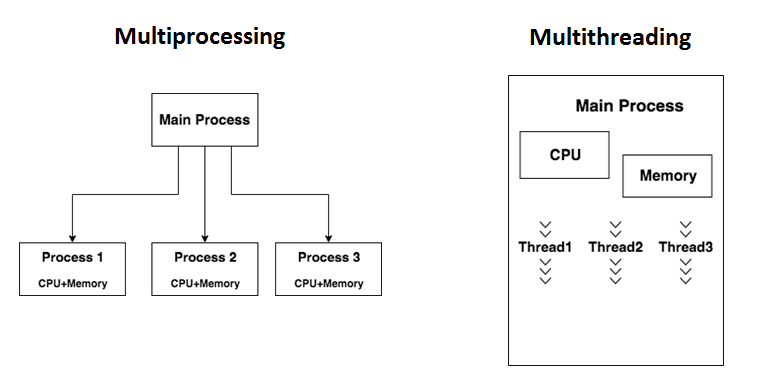
\includegraphics[width=0.8\textwidth]{threadvsmulti.png}
    \caption{Multiprocessing vs Multithreading}
    \label{fig:thread-vs-multiprocessing}
\end{figure}

